\chapter{Introduction}

%Pr: 3. St : 2
%why go to high  resolution -> several examples (bh relations - HST, HL TAU-ALMA, bullet cluster - chandra??) of how an increase in resolution has lead to new physical insights. 

Throughout the history of astronomy, we see celestial sources which appear point-like or unresolved with the instrumentation available at the time. To study these sources in enough detail to clarify their nature, ever more sophiscated instruments have to be developed. 

These instruments span the electromagnetic spectrum, and here I recall several notable examples which illustrate the discovery potential of an increase in resolution.

At optical wavelengths, the Hubble Space Telescope was able to resolve the gravitational sphere of influence of the central supermassive black hole (SMBH) in nearby galaxies. These measurements uncovered the fundamental relations between black hole mass and both stellar bulge luminosities and velocity dispersions (Ferrasse and Merritt (2000), Gebhardt et al. (2000)) which has been a foundation for extra-galactic astronomy ever since. 

A more recent example is a 2014 science verification result with the Atacama Large Millimetre Array (ALMA) \cite{brogan_2015} which resolves the molecular dust disk surrounding the young protostellar system, HL Tau Fig.~\ref{fig:hl_tau}. This observation showed, in unique detail, the orbit cleared out by forming planets which was suprising given that the stellar system was so young. The clarity of the image surpasses all previous work on the subject and provides an strong science case for conducting observations of similiar systems with ALMA. 

\begin{figure*}
\begin{center}

\includegraphics[width=1.4\columnwidth]{../../images/hltau}
\caption{The young stellar system HL Tau, observed at 223 GHz by ALMA. The orbits of forming planets appear as dark rings cut out of the disk. The presence of these bodies are suprising given that host star is still very young. The detail in this image was made possible by the milliarcsec resolution acheivable with ALMA. \label{fig:hl_tau}}

\end{center}
\end{figure*}

X-ray wavelengths with Chandra, we see the bullet cluster (Clowe 2004, )

The technique which acheives the highest resolution is Very Long Baseline Interferometry (VLBI)

\subsection{Very Long Baseline Interferometry}
%Pr : 3 St :3
% brief historical context of vlbi 

VLBI is  network 

The development of VLBI, originated in the late 1960's with observations of compact, highly-variable objects, now known as quasars. Teams using VLBI discovered that these objects consist of core-jet systems. Also the presence of super-luminal jet motion. \textit{TMS copy, paste : By using local
oscillators at each antenna that are controlled by high-precision frequency stan-
dards, it is possible to preserve the coherence of the signals for time intervals
long enough to measure interference fringes. The received signals are converted
to an intermediate frequency low enough that they can be recorded directly on
magnetic tape, and the tapes are subsequently brought together and played into
a correlator.}

% examples of arrays, with their specs

Examples of Arrays : Very Long Baseline Array (VLBA) : 1.4 - 87 GHz, European VLBI Network (EVN), African VLBI Network (AVN).  

\subsection{The Event Horizon Telescope (EHT)}
%Pr : 3, St: 3
This thesis is centred around such a class of emerging early 21st century instrumentation, known as Very Long Baseline Interferometry at millimetre wavelengths (mm-VLBI). This technique enables angular resolution on the order of $\sim 10\ \mu$-arcsec by maximising both antenna separation and observing frequency. The sub-field is being led by the Event Horizon Telescope consortium (EHT), an international project whose primary objective is to resolve the supermassive black holes  (SMBH) located at the centre on our Galaxy, known as Saggittarius~A$^\star$ (Sgr~A$^\star$), and M87 on angular scales comparable to the black hole event horizon. This thesis aims to contribute to the EHT objectives through algorthimic development of data simulation and parameter estimation pipelines, which are particularly relevant given the significant calibration challenges faced by the project.

\begin{figure*}
\begin{center}
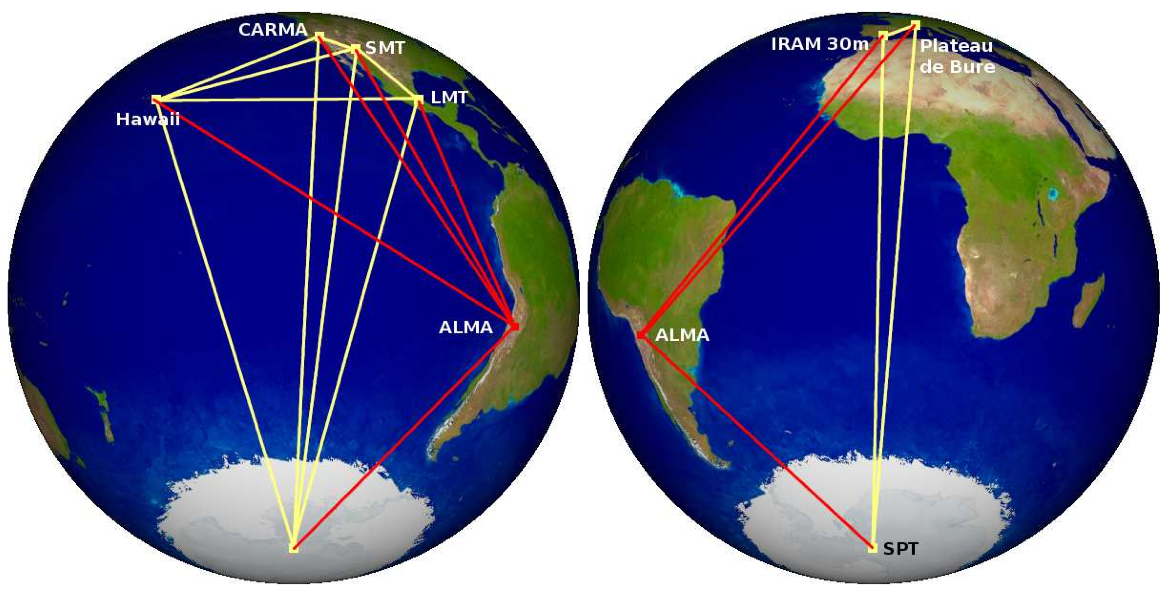
\includegraphics[width=1.4\columnwidth]{../../images/eht_globe}
\caption{(Image credit: Remo Tilanius) Event Horizon Telescope uses \textbf{Earth-diameter baselines} to attain \textbf{resolution} \boldmath$\sim 10$ $\mu$arcsec. \label{fig:eht_globe}%
}
\end{center}
\end{figure*}

\subsection{Scientific opportunities with the EHT}
%Pr : 3,  St:3
To constrain the physics near a black hole, the observation needs to be sensitive to scales comparable to the event horizon. For the case of a non-spinning or Schwarschild black hole, the event horizon is spherically symmetric with a radius, $R_{\rm Sch} = 2 G M_{\rm BH} /c^2$,  where $M_{\rm BH}$ is the black hole mass, $G$ is the gravitational constant and $c$ is the speed of light. The angular size of such an event horizon in the far field approximation is $\theta_{\rm Sch} = R_{\rm Sch} / D \approx 0.02$~nanoarcsec~($M_{\rm BH}/M_\dot$)(kpc/$D$) where $D$ is the distance from observer to source. For SMBH's Sgr~A$^\star$ and M87, this results in $\theta_{\Sch} \sim 5-10\ \mu$-arcsec. The event horizon telescope will have baseline lengths $|b| \sim 10^3$~km and is currently observing at $\nu =230$~GHz, yielding a diffraction-limited angular resolution of $\theta_{\rm EHT}$ = 1.22 \vu/ |b| \approx $. Hence EHT will be able to resolve these objects on the scale of the event horizon/gravitational radius. 

Equally important to  that the millimetre emission is optically thin and therefore probes inner emission region. The power spectrum of Sgr~A$^\star$ peaks in sub-mm bump. Synchtron emission. Lensed emission. the interferometric technique also filters out smooth mm emission.[Read Falke 1998]

{\bf FIG. basic grmhd image of black hole shadow, scale indicating resolution and eht beam size}\\


\subsubsection{Strong gravity and black hole spacetime}
%Pr : 3, St: 3
Gravity as described by General Relativity (GR) has flawlessly agreed with all observational experiments, however GR has conceptual weaknesses, especially as it is not compatible with the quantum description of reality. Various alternatives to GR have been theorised which do not assume a purely classical description of matter. To test GR against it's numerous alternatives, we have to observe gravity in the regime where we expect the largest observational deviations a GR prediction would have if it were only an approximate theory of gravity.  The spacetime close to a SMBH is an ideal candidate, as the gravitational effects are very strong. Lensed emission of the gravitational lensed photon ring.  The exact sizes and shapes of which indicate different spacetime and theories of gravity. Note that even in this regime, the deviation from GR is small. We can also explore black hole physics by testing the no-hair theorem or that black holes are only described by their mass, spin and charge by constraining the quadrapole moment of the black hole.deviations
from the Kerr metric

{\bf FIG. Plot of analytic shapes and sizes of the bh shadow from the predictions of different theories of gravity}\\
~\\
\subsubsection{AGN accretion and jet launch astrophysics} 

{\bf [AGN jet basics.]}

Astrophysical jets were first discovered over a century ago, accretion onto a black hole was first postulated to power these jet by .. .However a century later, the mechanism of accretion and jet launching ifrom SMBH are still highly debated. 

\textbf{Fig: Typical AGN jet illustration showing magnetic fields }

Recently an industry of sophiscated General Relativistic Magneto-Hydrodyanmic (GRMHD) simulations has developed yielding important insights but also new questions. Now, mm-VLBI has the opportunity of constrains the mechanisms. Specifically we can map the magnetic field configuration, which is a key aspect using polarimetry and Faraday Rotation. The quiescent and variability structure and also be explore in total intensity. Flaring structure.  Distiniguish between accretion disk and inner jet. Distinguish between the different Jet and Disk models for each bh. Deterimine spin.\\
~\\
\textbf{Fig: 2/3 panels of simulated images of disk and jet models of Sgr A*/M87}\\

In M87, where the jet is dominant, micro-arcsecond scale astrometry, capable with the EHT, can determine the distance from the jet base from the event horizon, as well as the width of the jet base. Opening up new possibilities in explore particle production and other exotic physics occuring at the event horizon. 


\textbf{Fig: 2/3 panels of simulated polarimetric images of Sgr A*/M87 showing ordered magnetic fields}
\subsection{Challenges and obstacles in mm-VLBI observations}
%Pr : 2, St : 2
Performing Very Long Baseline Interometry (VLBI) at mm-wavelengths presents unique calibration challenges, including very short atmospheric coherence times that are typically $\lesssim$10~s \citep{Doeleman_2009}, low calibrator source sky density, complex and variable calibrator source structure, and antenna pointing accuracies that are a non-negligible fraction of the antenna primary beam. Addition These effects may place significant limitations on the sensitivity, image fidelity, and dynamic range that can be achieved with mm-VLBI.  Performing mm-VLBI however, is a difficult task for a variety of reasons. Firstly the arrays are inhomogenous, made up of a collections of different stations working together, Difficult to get time on all the stations. there are a variety of signal corruptions which take place. Briefly introduce signal corruptions, variability, ..etc, how these represent calibration and interpretation challenges.


\subsection{Science extraction : parameter estimation and imaging}
%Leave for now
%Pr : 2, St : 3

Briefly discuss imaging, it's difficulties..\\we need to measure the fractional
asymmetry of the shadow shape with respect to its angular size to the few percent
~\\
Estimating the `macro'-parameters of Sgr A*, spin, orientation, position angle through a Bayesian parameter estimation analysis with closure quantities\\
Furthermore, unaccounted for systematic and/or non-Gaussian uncertainties could preclude robust, accurate Bayesian parameter estimation and model selection analyses of accretion flow \citep[e.g.][]{Broderick_2016} and gravitational physics \citep[e.g.][]{Broderick_2014, Psaltis_2016}, two of the EHT's many objectives.
~\\
\textbf{Fig: A Broderick 2016 posterior probability distribution (?)}

\subsection{A realistic mm-VLBI simulator}
%Pr : 1 : St : 2

%Why simulate: intro
Given the significant observation challenges that the EHT faces, we have undertaken this project to build a mm-VLBI observation and signal corruption simulator.  There are many benefits of such a toolkit and indeed synthetic data simulation is common practice for every major scientific experiment, with a recent example of gravitational wave template matching for LIGO (ref) or the extensive synthetic data generation for LHC particle collision experiments (ref).  In essence such a simulator would bridge the divide between physics governing the region associate with the source (e.g. SMBH) and the raw data, hence completing the link in the theoretical signal propagation chain. The remainder of this section will briefly discuss the variety of use cases for an EHT synthetic data simulator and how we have designed the software to meet these requirements. 

%Specific use cases of simulations
A key observational use case is the testing of calibration, parameter estimation and imaging algorithms and strategies. As the inputs to the simulator are known exactly, when passing simulated data through the data processing pipelines, we are better able to explore sources of error which would otherwise be impossible to disentangle from intrinsic source features.  A straightforward way to perform such a test is through the simulation of a set of `standard challenges' . Such datasets would then be calibrated and/or imaged with a variety of algorithms and routines which should identify comparative benefits and drawbacks.   


This be especially useful to explore unknown systematic errors which could be present in the signal processing chain and if unaccounted, could preclude robust, accurate Bayesian parameter estimation and model selection analyses of accretion flow \citep[e.g.][]{Broderick_2016} and gravitational physics \citep[e.g.][]{Broderick_2014, Psaltis_2016}, two of the EHT's objectives.




Through the eventual construction of an end-to-end pipeline, realistic synthetic data can be fit to observations, effectively reversing the simulator to perform calibration and parameter estimation. 

This contributes to theory through better determination of the scientific capabilities of the available instrumentation and measurement techniques.



[doeleman 2009]
Another use case for observations is that critical resources (such as stable frequency standards, high-bandwidth recording equipment, and phased-array processors) are likely to be limited initially, and telescope upgrades (such as surface accuracy improvement, expanded IF bandwidth, additional receiver bands, and simultaneous dual-polarization capability) must necessarily be prioritized. Simulated observational data can help assess the tradeoffs that must be considered for optimization of Galactic Center VLBI observations.



While \textsc{MeqTrees} has not yet been used in the context of mm-wavelength observations, the framework is agnostic to higher frequency implementation as long as the Measurement Equation is appropriately constructed. \textsc{MeqSilhouette} enables realistic interferometric simulations of mm-VLBI observations in order to gain deeper understanding of a wide range of signal propagation and calibration effects. 
leverage metre and cm-wavelength simulation and calibration successes and build a \textsc{MeqTrees}-based mm-VLBI-specific software package called \textsc{MeqSilhouette}. 


%what the thesis will do
This thesis will describe the software package along with its main features that include the capability to simulate tropospheric, ISM scattering, and time-variable antenna pointing error effects. 

This technology enables us to understand a wide range of mm-VLBI signal propagation and calibration systematics, quantify their effect on accretion flow and gravitational theoretical model selection, and hence maximise the scientific utility from EHT observations. 




























